\documentclass{mcmthesis}
\mcmsetup{CTeX = false,   % 使用 CTeX 套装时,设置为 true
        tcn = 55869, problem = E,
        sheet = true, titleinsheet = true, keywordsinsheet = true,
        titlepage = false, abstract = true}
\problem{E}

\usepackage{palatino}
\usepackage{mwe}
\usepackage{graphicx}
\usepackage{tabularx}
\usepackage{float}
\usepackage{indentfirst}
\usepackage{amsmath}
\title{}
\date{}

\begin{document}

\begin{abstract}%摘要


\indent  In recent years, with he rapid development in economy and explosive growth in population, environment pollution and depletion of resources have been aggravated day by day. Smart Growth was then put forward. Lots of cities have drawn up the development plans on basis of the combination of ten principles for Smart Growth and their own conditions. Our work is to evaluate the success of each city in Smart Growth and provide a guidance for plan making.Meanwhile, we need to measure the success of our smart growth plan. Therefore, we define the "Smart Growth Index" (SGI) to measure the success of smart growth and development plans of a city. \\
\indent  Our model establishes a Detail group of 52 indictors, which reflects the ten principles for smart growth and the three E's of sustainability. On basis of this, we can assess the success of smart growth of a city. In the construction of SGI model, we use linear aggregation to combine individual variables into the theme scores. Compensability of linear aggregation ensures fair assessment of different cities which have different emphasis in urban development. Then we use geometric aggregation to combine theme scores into SGI. Low compensability of geometric aggregation requires a city to develop evenly in all themes. We use entropy method to determine weights of indictors or themes, which avoid subjectivity. SGI model has an all-round and objective assessment of the success of smart growth of a city.\\
\indent  With the completion of these, we respectively select a city in China and America (Zhenjiang and Columbia.SC). We assess the success of city development and their smart growth on basis of SGI model. 
Finally, we proved the reasonability and applicability of our model.\\
\begin{keywords}
 {\bf{Geometric and linear aggregation ;  entropy method} }\par
\indent\indent\indent\indent\indent {\bf Smart Growth Index ;  PCA}
\end{keywords}
\end{abstract}

\maketitle
\tableofcontents\thispagestyle{empty}
%设置页眉


\setcounter{page}{1}
%Section 1
\section{Introduction}
\subsection{Background}%subsection 1.1

\subsection{Our work}


%Section 2
\section{Assumptions}
\noindent
{\bf (1) } The real change of indictors corresponds to policies.\\

\section{Symbol Description}
\begin{table}[h]
        \setlength{\abovecaptionskip}{0pt}
        \setlength{\belowcaptionskip}{0pt}
        \centering{Table 1:Notation} \\
        \begin{tabular}{p{3cm}|p{3cm}|p{6.6cm}}
        \hline
        \rowcolor[gray]{0.9}\bf{Symbol}	&\bf{uint}      &\bf{Meaning}\\
        \hline
        $S_{1}$		& $m^2  $		 & The top surface area of the bathtub 	\\
        $S_{2}$		& $m^2  $		 & The bottom surface area of the bathtub 	\\
        $S_{3}$		& $m^2  $		 & The side surface area of the bathtub 	\\
        \emph{S}	& $m^2  $		 & The surface area of the body\\
        \emph{h}	& $cm	$        & height of a person \\
        \emph{w}	& $kg	$        & weight of a person \\
        \hline
        \end{tabular}
        \end{table}

%Section 3
\section{Heat Dissipation Model}
In order to analyze the situation of heat dissipation. 
We first analyze the bathtub.\\
\indent The effect of a bathtub on heat loss is mainly in material and shape.\\
Because different bathtubs have different shapes and attributes, We use functions to describe the relationship between the surface area, the surface height and the volume of the surface area.
\begin{equation}
\begin{split}
h=H(v)  \\
S_{1}=S_{1}(v) \\
S_{2}=S_{2}(v)  \\
\end{split}
\end{equation}


\subsection{Liquid surface heat loss model}%subsection 3.1理论框架

\section{Model of hot water addition}
\subsection{Changes in the volume of water in a bathtub}

\subsubsection{People take the initiative to drain through the drain of the bathtub}

\subsubsection{Water overflow through the upper drain}
\section{Factors that affect the model}
\subsection{The effect of human body and body temperature on the model}
%subsection 4.1
We improved our model in view of the human body influence. Our improvement is mainly in the following aspects.
\subsubsection{The influence of the heat conduction}%sub subsection 4.1.1
The interior of the body is basically maintained at a constant temperature, and the temperature of the skin is close to the water in bathtub. So we can simplify the question.The simplified question is illustrated as floows.\\

\begin{figure}[H]
\centerline{\includegraphics[height=6cm]{skin.png}}
\caption{Heat conduction model of human body}
\label{skin}
\end{figure}
\indent We can assume that the temperature of the skin is the same as the water. We select the temperature of the rectum about 37.5 degrees as the body temperature. The problem can be simplified as the skin heat dissipating to the interior of the body.\\
\indent So we can use {\bf Newton's law of cooling} to calculate the speed of heat dissipation.\\
\begin{equation}
\begin{split}
\Delta T&=|T_{w}-T_{f}| \\
q&=h\Delta T	\\
\phi &=qA=Ah\Delta T
\end{split}
\end{equation}
\indent Where \textbf{\emph{q}} is the heat flux density. \textbf{\emph{h}} is the convection heat transfer coefficient of matter. \textbf{\emph{$\phi$}}  is heat transfer power (or heat transfer per unit time). \textbf{\emph{A}} is the heat transfer area.\\
\indent The surface area of the human body can be calculated by the following formula.
\begin{equation}
S= \begin{cases} & 0.0057*h+0.0121*w+0.0820\text{( man )} \\ & 0.0073*h+0.0127*w-0.2106\text{(woman)} \end{cases}
\label{s}
\end{equation}
\indent According to formula \ref{skin}, the quantity of heat dissipated($dQ$) in unit time is:
\begin{equation}
	\frac{\mathrm{d} Q}{\mathrm{d} t}=\phi =qA=Sh\Delta T
	\label{Q_skin}
\end{equation}
where \emph{h}=1.48,${T_{f}}=37.5^{\circ}$. \\
\subsubsection{The influence of the body shape}
The volume of the person in the water affects the height of the liquid. In order to discuss the influence on the liquid surface conveniently. We use the weight to estimate the volume of the body. We use $\rho =1.06\times10^{3}kg/m^{3}$ as the density of the human body, so the volume can be calculated:
\begin{equation}
v=\frac{m}{\rho }=\frac{m}{1.06\times 10^{3}}(m^{3})
\end{equation}
%Section 5
\section{Solutions for tasks }
\subsection{Different shapes of the bathtub}
We model and analysis several different shapes of bathtubs.
\subsubsection{Bathtub based on ovals}
\begin{figure}[H]
\centerline{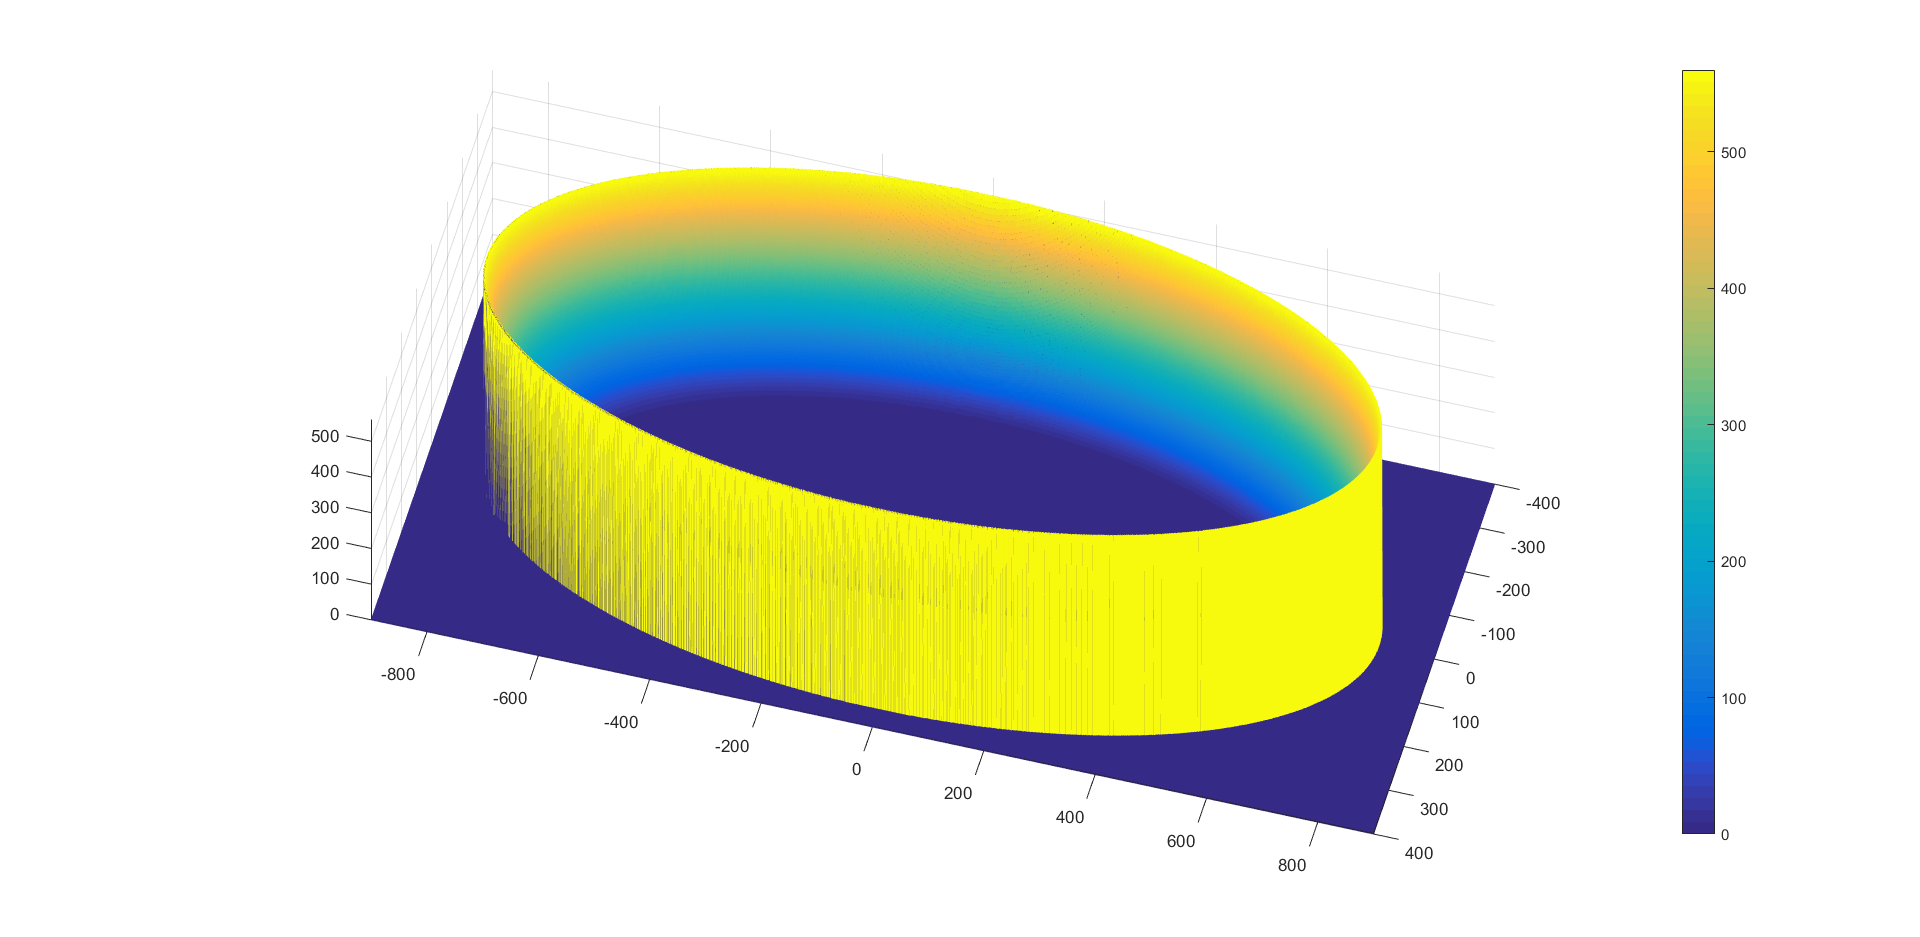
\includegraphics[height=8cm]{oval.png}}
\caption{The shape of bathtub based on ovals}
\label{oval}	
\end{figure}

\subsubsection{Bathtub based on circles}
\begin{figure}[H]
	\centerline{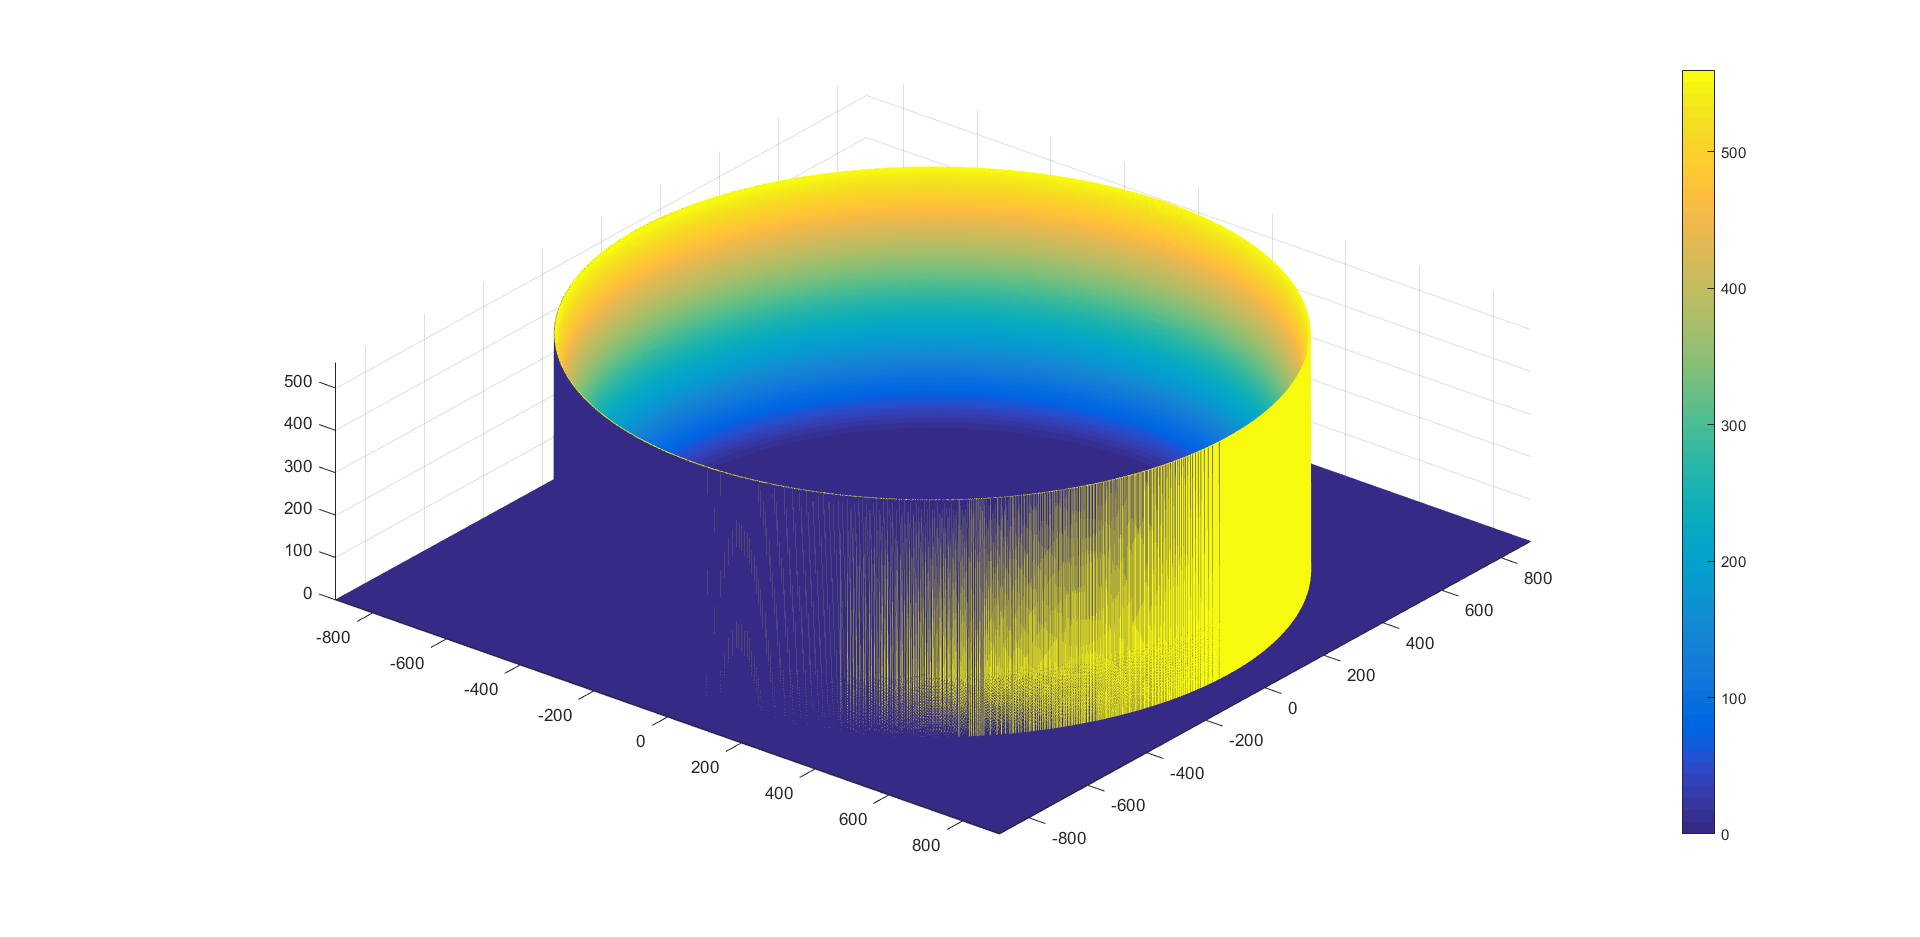
\includegraphics[height=8cm]{circle.png}}
	\caption{The shape of bathtub based on circles}
	\label{circle}	
\end{figure}

\subsection{Task 2}%subsection 5.2

According to the current researches on urban planning of our chosen cities (Columbia.SC and Zhenjiang), we adopt quantization analysis of plans or policies. Then we obtain the following policy conclusion:\\
%%政府政策
\begin{table}[h]

\centering
\centering{Table 2:Current Plan}
\begin{tabular}{p{5.2cm}|p{1.2cm}|p{5.2cm}|p{1.2cm}}
\hline
\bf Zheiang 5 years	 & \bf change	 & \bf Columbia 5 years	& \bf change \\
\hline
 per capita GDP(yuan/person)	& +8\%	& per capita disposable income( yuan)	& +5\% \\
production of tertiary industry ratio(\%)	& to 50\%	& per capita green spaces($m^2$)	& +4\% \\
per capita disposable income(yuan)	& +8.5\%	& average wages of staff(yuan)	& +5\% \\
tourist income ratio in GDP(\%)	& +100\%	& sewage treatment ratia(\%)	& to 99\% \\
total export(100 million dollars)	& +50\%	& high school enrollment(10000 person)	& +8\% \\
amount of doctors (per ten thousand)	& +10\%	& per capita living space($m^2$)	& +7\% \\
per captia area of roads(urban,$m^2$)	& +10\%	& green cover in built up area(\%)	& +5\% \\
\hline
\end{tabular}
\end{table}

\noindent Using SGI model, we can obtain SGI of two cities after implementing the current plan. Also, we can obtain original SGI on the basis of original data. Based on the method in section 4, we can get the following result by way of matlab.\\

%%政府政策中SGI总和
\begin{table}[h]
\setlength{\abovecaptionskip}{0pt}
\setlength{\belowcaptionskip}{0pt}
\centering{Table 3:SGI of Current Plan}
\begin{tabular}{p{3.3cm}|p{3cm}|p{3cm}|p{3.3cm}}
\hline
City	& $SGI_0$ (2014)	& $SGI$ (2020)	& $\Delta SGI$ \\
\hline
Zhenjiang	& 12.5126	& 14.3771	& 1.8645 \\
columbia	& 13.962	& 14.1089	& 0.1469 \\
\hline
\end{tabular}
\end{table}
%%
\noindent Through the analysis of the relative change in SGI of two cities, we can assess the success of the growth plan.\\
Apparently, SGI of two cities both increases after implementing their own current growth plan. \\
Thus, their current growth plan is both successful.\\
\subsection{Task 3}%subsection 5.3
\subsubsection{Our growth plans}%sub subsection 5.3.1
Combining the current plans of two cities and ten principles of smart growth, we make the following growth plans for our cities over few decades.\\
%%我们的计划
\begin{table}[h]
\setlength{\abovecaptionskip}{0pt}
\setlength{\belowcaptionskip}{0pt}
\centering{Table 4:Our Plan}
\begin{tabular}{p{5.3cm}|p{1.2cm}|p{5.2cm}|p{1.2cm}}
\hline
\bf Zhenjiang 10 years	& \bf change	 & \bf Columbia 10 years	& \bf change \\
\hline
 per capita GDP(yuan/person)	& +100\%	& per captia area of roads(urban,$m^2$)	& +15\% \\
production of tertiary industry ratio(\%)	& to 55\%	& ability of harmless treatment planet(ton)	& +100\% \\
total export(100 million dollars)	& +100\%	& tourist income ratio in GDP(\%)	& +100\% \\
per capita disposable income(yuan)	& +100\%	& amount of professionals(10000 person)	& +50\% \\
 per capita green spaces($m^2$)	& +20\%	& expenditure in education ratio in GDP	& to 10\% \\
 high school enrollment(10000 person)	& +100\%	& high school enrollment(10000 person)	& +50\% \\
total social labor productivity(yuan)	& +200\%	& amount of ward beds(per ten thousand)	& +30\% \\
amount of ward beds(per ten thousand)	& +20\%	& per capita green spaces($m^2$)	& +10\% \\
\hline
\end{tabular}
\end{table}

%%
\subsubsection{Reasons for choosing these initiatives}%sub subsection 5.3.2
Ten principles of smart growth can be reflected in the detailed of indictors. Thus, in the process of making our smart growth plans, we just need to choose appropriate indictors supported by policies on basis of geography and economic development.\\

\noindent For Zhenjiang, as manufacturing industry basement in middle and lower reaches of Yangtze River in China, adept in manufacturing and export, we can stimulate its export in our plan, which can accelerate the development of city. Even though economic development is on the agenda, the environment and medical level is as important as economic development. Thus, we also give priority to relative indictors of these elements in our smart growth plan. \\
For Columbia.SC, its economy and livelihood have higher level, thus we put its emphasis on education, technology and protection of environment. In the meanwhile, tertiary industry should be developed rapidly, which plays important role in urban development. \\
\noindent Therefore, we make these smart growth plans above for both cities. \\
\subsubsection{Assessment of the success of our smart growth plans}%sub subsection 5.3.3
Based on the method in task 2, we can obtain the changes in SGI of two cities by way of matlab after implementing our growth plans.\\
%%我们的计划中SGI总和
\begin{table}[h]
\setlength{\abovecaptionskip}{0pt}
\setlength{\belowcaptionskip}{0pt}
\centering{Table 5:SGI of Our Plan}
\begin{tabular}{p{3cm}|p{3cm}|p{3cm}|p{3cm}}
\hline
City	& $SGI_0$ (2014)	& $SGI$ (2025)	& $\Delta SGI$ \\
\hline
Zhenjiang	& 12.5126	& 15.4329	& 2.9023 \\
columbia	& 13.962	& 15.092	& 1.13\\
\hline
\end{tabular}
\end{table}

%%
\noindent Apparently, SGI of two cities both increases after implementing our smart growth plan. Therefore, our smart growth plans are successful in the chosen cities through analysis.\\
\subsection{Task 4}%subsection 5.4
\subsubsection{Assessment of the importance of each initiative}%sub subsection 5.4.1
In this task, we need to rank our chosen initiatives of our smart growth plan. Thus, we can compare the importance of each initiative to complete this task.\\
On basis of the method mentioned in 4.2 of section 4 and SGI model, we can obtain the   following ranking of each city by way of matlab.\\
%%计划排名
\begin{table}[h]
\setlength{\abovecaptionskip}{0pt}
\setlength{\belowcaptionskip}{0pt}
\centering{Table 6:Ranking of initiatives}
\begin{tabular}{p{1cm}|p{7cm}|p{1.3cm}|p{1.4cm}|p{1.4cm}}
\hline
\hline
\rowcolor[gray]{0.9}\multicolumn{5}{c}{Columbia}\\
\hline
\bf rank & \multicolumn{2}{|c|}{ \bf  initiatives} & \bf SGI	&  \bf $\Delta SGI$ \\
\hline
1	& tourist income ratio in GDP(\%)	& +100\%	& 14.3194	& 0.3574 \\
2	& high school enrollment(10000 person)	& +50\%	& 14.2334	& 0.2714 \\
3	& ability of harmless treatment planet(ton)	& +100\%	& 14.1711	& 0.2090 \\
4	& amount of professionals(10000 person)	& +50\%	& 14.0586	& 0.0966 \\
5	& expenditure in education ratio in GDP	& to 10\%	& 13.9929	& 0.0309 \\
6	&  amount of ward beds(per ten thousand)	& +30\%	& 13.9838	& 0.0218 \\
7	& per capita green spaces($m^2$)	& +10\%	& 13.9811	& 0.0190 \\
8	& per captia area of roads(urban,$m^2$)	& +15\%	& 13.9726	& 0.0106 \\
\hline
\hline
\rowcolor[gray]{0.9}\multicolumn{5}{c}{Zhenjiang}\\
\hline
\bf rank & \multicolumn{2}{|c|}{ \bf  initiatives} & \bf SGI	&  \bf $\Delta SGI$ \\
\hline
1	& total export(100 million dollars)	& +100\%	& 14.4935	& 1.9809 \\
2	&  high school enrollment(10000 person)	& +100\%	& 13.0236	& 0.5109 \\
3	& per capita disposable income(yuan)	& +100\%	& 12.6755	& 0.1628 \\
4	& total social labor productivity(yuan)	& +200\%	& 12.6102	& 0.0975 \\
5	&  per capita GDP(yuan/person)	& +100\%	& 12.5504	& 0.0377 \\
6	& amount of ward beds(per ten thousand)	& +20\%	& 12.5304	& 0.0177 \\
7	&  per capita green spaces($m^2$)	& +20\%	& 12.5288	& 0.0161 \\
8	& production of tertiary industry ratio(\%)	& to 55\%	& 12.5128	& 0.0002 \\
\hline
\end{tabular}
\end{table}

%%
\subsubsection{Analysis of the ranking}%sub subsection 5.4.2
Evidently, the ranking proves the reasonability of our plans' emphasis.\\
The ranking of the same initiatives of both cities is the same (education, medical level and green spaces). Thus, each of these indictors play the same role in urban development.  
Giving thought to national conditions of both cities, Zhenjiang's emphasis is economic development while Columbia's is soft strength of society like education, as well as technology and tertiary industry. The ranking of each city's initiatives is correspond to our reasons for choosing these initiatives. \\
\subsection{Task 5}%subsection 5.5
In the case of that the population of city will increase 50\% by 2050, we analyze our group of indictors. We find that the increase of population has negative effects on population density, per capita green spaces and per capita living space so on.\\
Due to population density and per capita living space not under the control of governmental policies or plans, we neglect these indictors in our smart growth plan.\\
For Columbia.SC and Zhenjiang there are several initiatives like $per$ $capita$ $green$ $spaces$ and $amount$ $of$ $ward$ $beds(per$ $ten$ $thousand)$\\
These implements all can effectively curb the negative impacts of the increase of population. \\

%Section 6
\section{Sensitivity analysis}
\subsection{Selection of indictors}%subsection 6.1
The aim of this analysis is to determine whether a single variable had an unduly large impact on the overall ranking. To test this, we randomly exclude variables/themes from the index several times. The rest of variables/themes can use the same method to aggregation smart growth index (SGI). Observe and analyze the distribution of SGI of two cities.\\
%%盒型图
\centerline{\includegraphics[height=8cm]{boxplot.png}}
\centerline{Figure2:boxplot}
As is shown in the figure of statistics, the SGI of Columbia.SC is generally higher than that of Zhenjiang. The SGI of Zhenjiang is more sensitive to that of Columbia.SC. The result proves that SGI of Zhenjiang benefits from some indictors in degrees. In other words, the development of Columbia.SC is more balanced than that of Zhenjiang.\\
\subsection{Selection of aggregation method}%subsection 6.2
In Task 1, we compare linear aggregation with geometric aggregation in advantages. For that reason, we finally decided to use linear aggregation to combine individual variables into the theme scores and geometric aggregation to combine theme scores into SGI.\\
We tried to use geometric aggregation to combine individual variables into the theme scores. And we observe that the calculated SGI using different data may varies in difference.\\
Our model is sensitive to the selection of aggregation method.\\

%Section 7
\section{Strengths and weaknesses}
\subsection{Strengths}%subsection 7.1
\begin{itemize}
\item Our model establishes a detailed group of 52 indictors, which reflects the ten principles for smart growth and the three E's of sustainability. On basis of this, we can assess the success of smart growth of a city.
\item In the construction of SGI model, we use linear aggregation to combine individual variables into the theme scores. Compensability of linear aggregation ensures fair assessment of different cities which have different emphasis in urban development. Then we use geometric aggregation to combine theme scores into SGI.Low compensability of geometric aggregation requires a city to develop evenly in all themes. 
\item We use entropy method to determine weights of indictors or themes, which avoid subjectivity.
\item SGI model has an all-round and objective assessment of the success of smart growth of a city.
\end{itemize}
\subsection{Weakness}%subsection 7.2
\begin{itemize}
\item In our model, we regard the relationship between initiative and indictor as one to one. In reality, a plan can result in the change in other indictors(not included in plan) because of correlation between indictors. The real SGI may be different with our calculated SGI.
\item In our model, we neglect the government's executive force.
\end{itemize}


\section{References}
\begin{thebibliography}{99}
\bibitem{1}Bannerjee,S.Bone,J.and Finger,Y.(2016).European Digital City Index-Methodology Report.Nesta Report-ISBN Number:978-1-84875-153-8
\bibitem{2}\url{http://www.wolframalpha.com/input/?i=columbia,+sc}
\bibitem{3}Jing Tan,Xiaoma Tao,Xu Chen.(2012).A Synthetic Measurement of Urban "Smart Growth" Based on Improved Entropy Method.Resources and Environment in the Yangtze Basin
\bibitem{4}Zhenjiang Statistical Yearbook,2014. Available at:\\
\url{http://tjj.zhenjiang.gov.cn/tjzl/tjnj/}
\bibitem{5}National Bureau of Statistics of China. Available at:\\
\url{http://data.stats.gov.cn/}
\bibitem{6}Data of Columbia.SC. Available at:\\
\url{http://www.city-data.com/city/Columbia-South-Carolina.html}
\bibitem{7}Yujuan Chen,Qifen Zha,Xiaolan Li.(2006).Application of Entropy Method in the Evaluation of Urban Sustainable Development.Journal of Jiangsu University(Social Science Edition)
\end{thebibliography}

\begin{appendices}
Here are  programmes we used in our model as follow.\\
\textbf{\textcolor[rgb]{0.98,0.00,0.00}{calculation of SGI matlab source:}}
\lstinputlisting[language=Matlab]{./code/model.m}
\textbf{\textcolor[rgb]{0.98,0.00,0.00}{calculation of weight by the entropy method matlab source:}}
\noindent{\lstinputlisting[language=Matlab]{./code/entropy.m}}
\end{appendices}

\end{document}